\documentclass[11pt,a4paper]{article}

\usepackage[T1]{fontenc}
\usepackage[utf8]{inputenc}
\usepackage[margin=1in]{geometry}
\usepackage{graphicx}
\usepackage{booktabs}
\usepackage{array}
\usepackage{amsmath,amssymb}
\usepackage[font=small,labelfont=bf]{caption}
\usepackage{microtype}
\usepackage[hidelinks]{hyperref}
\usepackage{xcolor}
\hypersetup{colorlinks=true,linkcolor=blue,citecolor=blue,urlcolor=blue}

\graphicspath{{figures/}}
\setlength{\parskip}{2pt}
\setlength{\parindent}{0pt}
\renewcommand{\arraystretch}{1.12}

\title{Faster, not better: mapping the anytime efficiency\\[2pt]
and boundaries of short-period learning-rate cycles}
\author{Anonymous Authors}
\date{Draft --- Revision B}

\begin{document}
\maketitle

\begin{abstract}
We study what a learning-rate schedule buys when it is evaluated as an \textbf{anytime algorithm} rather than only at the end of training. The schedule composes two established components in two lines of code: Smith's triangular cycle, shortened to a period of one epoch, multiplied by a cosine anneal. Neither component is new and we claim no novelty for the composition. On CIFAR-10 with ResNet-18, momentum-free SGD at a peak learning rate of 0.8 reaches 90\% test accuracy in \textbf{16.7 epochs}, against \textbf{68.7} for a mean-matched cosine control (same average learning rate, no cycle; 4.1x sooner, paired t = 11.53, 3/3 seeds) and \textbf{107.7} for the standard momentum-0.9 recipe (6.5x sooner, t = -78.8), at final accuracy with no detectable difference. On CIFAR-100 the same comparison gives 5.5x/5.3x sooner to 65\%/70\%. We then map the boundaries of the effect: it is concentrated in early-to-mid training and becomes negligible near each dataset's accuracy ceiling (95\% on CIFAR-10, 75\% on CIFAR-100). It requires momentum-free SGD --- adding momentum 0.9 costs 2.8 points and 142 epochs --- and shows no detectable benefit on AdamW at the tested configuration (-0.33 pp, n.s.). We additionally report a methodological observation for practitioners: in our runs, an LR-independent weight-decay coefficient collapsed to chance in the final epochs (final loss essentially ln 10 = 2.3026), while both LR-coupled conventions did not. Because the constant arm was also 2.5x/5x stronger on average, the collapse cannot be attributed to the decay profile alone; we state it as a caution and an open confound. Our contribution is a controlled characterisation of a short-period regime and its failure modes, not an accuracy claim; we do not claim superiority over long training horizons.

\end{abstract}

\section{Introduction}
Most reported learning-rate discoveries combine a schedule change with a regime change and report only the final number, which makes attribution hard. This paper reports a deliberately small observation and then spends most of its length trying to falsify it.

\textbf{The observation.} Take a standard cosine anneal, multiply it by a triangular cycle whose period is one epoch, and run momentum-free SGD at a high peak learning rate. In a fixed 200-epoch budget, training reaches a given accuracy several times sooner than the standard recipes, at the same final accuracy.

We state the hypothesis before the evidence. The comparison is not ``is this schedule better than long training?'' --- at convergence it is not, and we do not claim that. The hypothesis is narrower:

\begin{center}
\small
\begin{tabular}{@{}>{\raggedright\arraybackslash}p{0.140\linewidth}>{\raggedright\arraybackslash}p{0.257\linewidth}>{\raggedright\arraybackslash}p{0.257\linewidth}>{\raggedright\arraybackslash}p{0.257\linewidth}@{}}
\toprule
\textbf{\#} & \textbf{skeptical hypothesis to be tested} & \textbf{test} & \textbf{outcome} \\
\midrule
H1 & the speed is explained by the lower average learning rate & mean-matched cosine control (\S{}5.1) & \textbf{rejected} --- 4.1x survives \\
H2 & the speed is an evaluation-timing artifact & half-epoch phase shift (\S{}5.3) & \textbf{rejected} --- no effect \\
H3 & the speed is an artifact of a fixed 200-epoch horizon & budget-matched runs 40/80/160 (\S{}5.2) & \textbf{rejected} --- the method wins at every budget (n=1, directional) \\
H4 & the advantage disappears against a tuned or momentum baseline & standard momentum-0.9 recipe; tuned AdamW (\S{}5.4, \S{}5.7) & \textbf{rejected} --- the gap grows to 6.5x; the AdamW margin halves but survives \\
H5 & the cycle changes final accuracy & paired tests on both datasets & \textbf{not rejected} --- ties within n=3 resolution \\
H6 & the effect is universal & threshold, dataset, optimizer and budget sweeps (\S{}5.2, \S{}5.6-\S{}5.7) & \textbf{rejected} --- it vanishes near each ceiling; AdamW shows no detectable benefit at the tested config (n.s.) \\
\bottomrule
\end{tabular}
\end{center}

Two negative results are part of the contribution rather than an apology for it. First, the schedule requires momentum-free SGD: the identical schedule at momentum 0.9 ends 2.8 points lower and reaches 90\% only at epoch 159. Second, in our runs an LR-independent weight-decay coefficient collapsed to chance in the final epochs, while LR-coupled decay did not; because the constant arm was also 2.5x/5x stronger on average, profile and strength are confounded, and we report this as a caution and an open question rather than a causal claim (\S{}5.8). The second result is useful to practitioners independently of the speed effect, and we give it a full section.

\textbf{A theoretical frame: the Edge of Stability.} A natural language for what a rapidly varying step size does comes from the Edge of Stability (EoS) literature. Cohen et al. \cite{ref6} show empirically that full-batch gradient descent on neural-network objectives typically operates in a regime where the largest eigenvalue of the training-loss Hessian hovers just above the numerical stability threshold $2/\eta$, with the loss non-monotone on short timescales but decreasing on long ones. Our schedule makes $\eta$ itself oscillate by a factor of 1000 within every epoch: at the start of training the stability threshold $2/\eta$ swings between roughly $2.5$ (at the peak $\eta = 0.8$) and roughly $2500$ (at the floor $8\times10^{-4}$), and the cosine envelope scales both down together. A one-epoch cycle therefore repeatedly enters and leaves the EoS regime instead of settling at one operating point. This is a promising explanation for why the schedule explores quickly without ending at a worse solution, and the momentum ablation is consistent with it, but we did not measure Hessian spectra. We use EoS as an interpretive hypothesis (\S{}6.2), not as a tested mechanism.

We claim no novelty for the schedule. The triangular cycle is Smith's cyclical learning-rate policy \cite{ref1}; the cosine anneal is Loshchilov \& Hutter \cite{ref2}; composing them is a two-line \texttt{LambdaLR}. Recommended cycles are far longer than ours: Smith recommends a half-cycle of 2-10 epochs (a full cycle of 4-20 epochs), and SGDR's T0=1 row is the only sub-2-epoch test, transient and confounded with doubling. No prior work isolates a fixed one-epoch period. Our contribution is the controlled characterisation of that regime, the boundary map that says when the effect appears and when it does not, and the negative results about what the effect is \textit{not}.

\textbf{Contributions.}

\begin{enumerate}
\item A rigorous hypothesis-test programme (H1-H6 above) that tries to explain away the observed speedup by matching the average learning rate, the evaluation phase, the compute budget, the baselines' tuning, and the baselines' momentum. The speedup survives all five; what does not survive is any claim about final accuracy.
\item A \textbf{boundary map} of short-period learning-rate dynamics: the effect is real but local in threshold, budget, optimizer and momentum (\S{}6.3). Establishing that a configuration is stable and competitive inside this ultra-short regime is itself a useful citable result.
\item A negative mechanistic result: the schedule requires momentum-free SGD, which constrains the class of explanations (\S{}5.5, \S{}6.2).
\item A methodological observation for training engineers: in our runs an LR-coupled, annealed weight decay survived the training tail while an LR-independent constant coefficient collapsed; the intra-epoch oscillation of the decay was \textit{not} required, and the strength/profile confound is stated explicitly (\S{}5.8).
\item A fully specified protocol with exact seed counts, paired tests, per-seed dispersion and regenerable tables and figures (\S{}4.2, \S{}8).
\end{enumerate}

\textbf{What we do not claim.} No accuracy advantage over tuned cosine annealing: final accuracy shows no detectable difference on either dataset, and the standard momentum recipe is 0.16 points \textit{ahead} on peak (a small, consistent deficit). No novelty in the schedule. No universal superiority, and no claim of being ``faster in wall-clock for equal total work''. The claim is time-to-a-given-accuracy inside a fixed epoch budget --- an anytime property.

\section{Related work}
\textbf{Cyclical learning rates.} Smith \cite{ref1} introduces triangular, triangular2 and \texttt{exp\_range} policies updated per iteration, and reports that a half-cycle of 2-10 epochs works well. Our cycle is one epoch --- the same mechanism, shorter than the recommended 4-20-epoch range. Smith's CIFAR-10 control (oscillating versus one-way decay at equal iterations, 81.4\% versus 78.5\%) is the closest published evidence for oscillation; it does not isolate a fixed sub-2-epoch period.

\textbf{Cosine annealing and warm restarts.} Loshchilov \& Hutter \cite{ref2} introduce SGDR, which anneals on a cosine and restarts periodically. We compose the cosine anneal \textit{with} the cycle and never restart: the anneal is monotone for the whole run. Super-convergence \cite{ref3} and the one-cycle policy \cite{ref4} similarly use a single large cycle; our regime is many short cycles inside one long anneal, which neither paper tests.

\textbf{Decaying schedules at scale.} Recent work argues for decay-dominated schedules: warmup-stable-decay / river-valley schedules \cite{ref10}, power schedulers \cite{ref11}, and compute-optimal training beyond fixed durations \cite{ref9}. Our result is consistent with that line in spirit --- the anneal supplies the final accuracy and the cycle supplies speed --- and our regime is the small-data, few-epoch vision regime where those large-scale findings need not transfer. We therefore position the paper as a regime study with a null hypothesis, not as evidence against decaying schedules.

\textbf{Edge of Stability.} Cohen et al. \cite{ref6} characterise EoS for full-batch GD; Jastrz\k{e}bski et al. \cite{ref7} relate large learning rates to traversing high-loss regions before descent; recent work \cite{ref8} connects large-LR implicit bias to EoS, balancing and catapult dynamics. Our schedule is a deliberate, repeated perturbation of the stability threshold $2/\eta$, which makes EoS the natural interpretive frame. We are explicit that this is an analogy: EoS theory is stated for fixed-step, full-batch GD, whereas we run mini-batch SGD with a rapidly varying step, and we do not measure sharpness.

\textbf{Metrics and protocol.} We report time-to-threshold (\texttt{t@X}) rather than only final accuracy, because a schedule can be anytime-better while asymptotically equal. The epochal-sawtooth phenomenon \cite{ref12} is a reminder that per-epoch loss oscillations can come from data reshuffling and adaptive optimizers rather than from the LR cycle; we report accuracy at a fixed evaluation phase and test the phase explicitly (\S{}5.3).

\section{Method}
\subsection{Schedule}
With \texttt{steps\_per\_epoch = 390} and \texttt{T = 200} epochs:

\begin{verbatim}
lr(t) = lr_max * tri((t mod spe) / spe) * cos_anneal(t / spe)

tri(x) = 2x          for x < 1/2      (scaled to [1/1000, 1])
       = 2 - 2x      otherwise
\end{verbatim}

\begin{figure}[htbp]
\centering
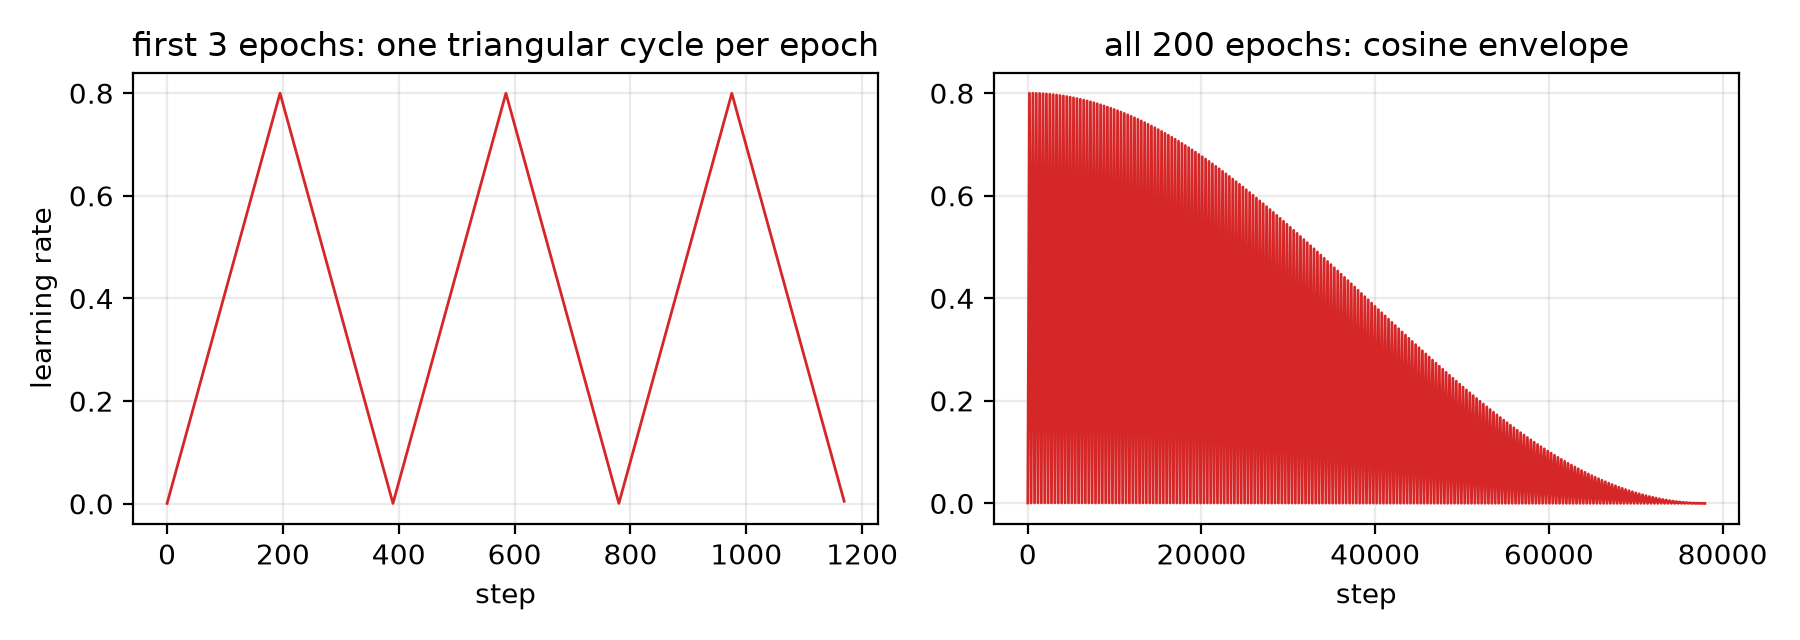
\includegraphics[width=0.92\linewidth]{figures/fig2_schedule.png}
\caption{The schedule. Left: the first three epochs, one triangular cycle per epoch. Right: all 200 epochs, showing the cosine envelope multiplying the cycle. The floor is $10^{-3}$ of the current peak; the anneal brings the peak to $10^{-4}$ of its initial value by epoch 200.}
\end{figure}

The method is stock PyTorch:

\begin{verbatim}
opt = torch.optim.SGD(params, lr=0.8, momentum=0.0, weight_decay=5e-4)
sched = torch.optim.lr_scheduler.LambdaLR(
    opt, lambda t: triangle(t % steps_per_epoch) * cosine(t / steps_per_epoch))
\end{verbatim}

No custom optimizer is in the method path. (A custom optimizer exists only to prove numerical equivalence to the stock composition; that check is an engineering decision helper and is not a paper result.)

\subsection{Weight decay convention}
\texttt{torch.optim.SGD} scales the decay coefficient by the current learning rate (\texttt{sgd.py}:355, :379), and \texttt{LambdaLR} keeps that learning rate current. The method therefore inherits an \textbf{LR-coupled, hence annealed, decay}, which \S{}5.8 suggests is the safer convention. We make this explicit here because the convention is easy to get wrong and its failure, when it occurs, is silent until the final epochs.

\subsection{Alignment consequence}
With a one-epoch cycle, every epoch boundary lands on the LR trough, so validation is always measured at the model's most stable phase. This is a potential confound and we test it directly in \S{}5.3.

\section{Experimental setup}
\subsection{Protocol}
CIFAR-10 and CIFAR-100 \cite{ref13} with ResNet-18 (CIFAR stem) \cite{ref14}, 200 epochs, batch 128 (390 optimizer steps per epoch), the full 50k training set, evaluation on the official 10k test split, plain augmentation (random crop + horizontal flip), no mixup, no EMA. All arms share this protocol; only the schedule and the optimizer differ. Runs take \textasciitilde{}20 s/epoch on an NVIDIA RTX A4000 and are resumable (\texttt{--skip-existing}).

\textbf{Metrics.} \texttt{t@X} is the first epoch at which test accuracy reaches X. Because CIFAR-100 tops out near 78\%, its thresholds are 65/70/75\%. All thresholds are reported in the tables rather than only the most favourable one.

\subsection{Seeds, pairing and statistical protocol}
This section exists because the paper's confidence claims depend on it, and because a small seed count can leave minor gaps underpowered.

\begin{itemize}
\item \textbf{Headline and ablation arms use $n=3$ seeds}, fixed and identical across arms (\texttt{seeds 0, 1, 2}). Seeds control initialization and data order, so comparisons are \textbf{paired by seed}; pairing removes between-seed variation from the comparison.
\item \textbf{Single-seed arms are labelled as such wherever they appear}: the constant-LR sweep (6 learning rates, 1 seed each), the budget-matched runs (40/80/160 epochs, 1 seed each), and the undertuned CIFAR-100 AdamW point (0.7283, 1 seed). Their results are directional, not significant.
\item \textbf{Tests.} Two-sided paired t-test by seed at $n=3$ ($\mathrm{df}=2$; the critical value for $p<0.05$ is $|t| \ge 4.303$, which we round to 4.30). We report the effect size, $t$, and the number of seeds on which the sign agrees, rather than only a p-value.
\item \textbf{Power.} With paired seed standard deviations of roughly 0.2 pp on accuracy, $n=3$ resolves differences of roughly 0.6 pp or larger at 80\% power. The headline final-accuracy tie has a paired s.d. of 0.28 pp, so its resolution is \textasciitilde{}0.8 pp. Differences below that are reported as \textbf{no detectable difference}, not as proof of equivalence. The three final-accuracy ties in this paper (mean-matched CIFAR-10: +0.14 pp, $t=0.90$; mean-matched CIFAR-100: -0.20 pp, $t=-1.48$; standard recipe: -0.17 pp, $t=-1.53$) are all in this underpowered region, which is why we describe them as ties \textit{within the resolution of three seeds} and not as exact equality.
\item \textbf{Replication status by result} is summarised below; any claim not carried by a $n=3$ paired test is marked directional.
\end{itemize}

\begin{center}
\small
\begin{tabular}{@{}>{\raggedright\arraybackslash}p{0.260\linewidth}>{\raggedright\arraybackslash}p{0.217\linewidth}>{\raggedright\arraybackslash}p{0.217\linewidth}>{\raggedright\arraybackslash}p{0.217\linewidth}@{}}
\toprule
\textbf{result} & \textbf{arms} & \textbf{seeds} & \textbf{status} \\
\midrule
CIFAR-10 speed, thresholds, final accuracy & method, mean-matched cosine, standard recipe & 3 & paired tests \\
CIFAR-100 speed, thresholds, final accuracy & method, mean-matched cosine, peak-0.2 cosine & 3 & paired tests \\
Momentum ablation (method + momentum) & 4 arms & 3 & paired tests \\
AdamW comparison and tuning grid & lr x wd grid on CIFAR-10 & 3 & paired tests \\
Weight-decay conventions (E2) & B1/B2/F & 3 & paired tests; strength confound open (\S{}5.8) \\
Evaluation-phase shift & method at trough vs peak & 3 & paired tests \\
Ablation: cycle without anneal & 1 arm & 3 & paired tests \\
Constant-LR sweep & 6 learning rates & \textbf{1} & directional \\
Budget-matched runs & 2 arms x 3 budgets & \textbf{1} & directional \\
CIFAR-100 AdamW undertuned point & 1 arm & \textbf{1} & directional (0.7283) \\
Peak-LR sensitivity \{0.4, 1.2\} & --- & --- & \textbf{not run} (limitation \S{}7) \\
\bottomrule
\end{tabular}
\end{center}

\subsection{Figures and variance}
Every learning-curve figure (Figs. 2 and 4) plots the \textbf{mean of the three seeds with a shaded $\pm 1$ s.d. band}; curves are smoothed with a 3-epoch moving average so the figure shows trends rather than evaluation-to-evaluation noise. The bands are visible throughout and widen near each dataset's ceiling, which is one of the observations the boundary claim rests on. Fig. 3 (time-to-threshold bars) carries \textbf{$\pm 1$ s.d. error bars across the three seeds}; the E2 figure uses the mean and per-seed range. The figures are descriptive; all significance statements are computed on per-seed values, not from the smoothed curves.

\section{Results}
\subsection{Speed, against a mean-matched control (CIFAR-10)}
\begin{figure}[htbp]
\centering
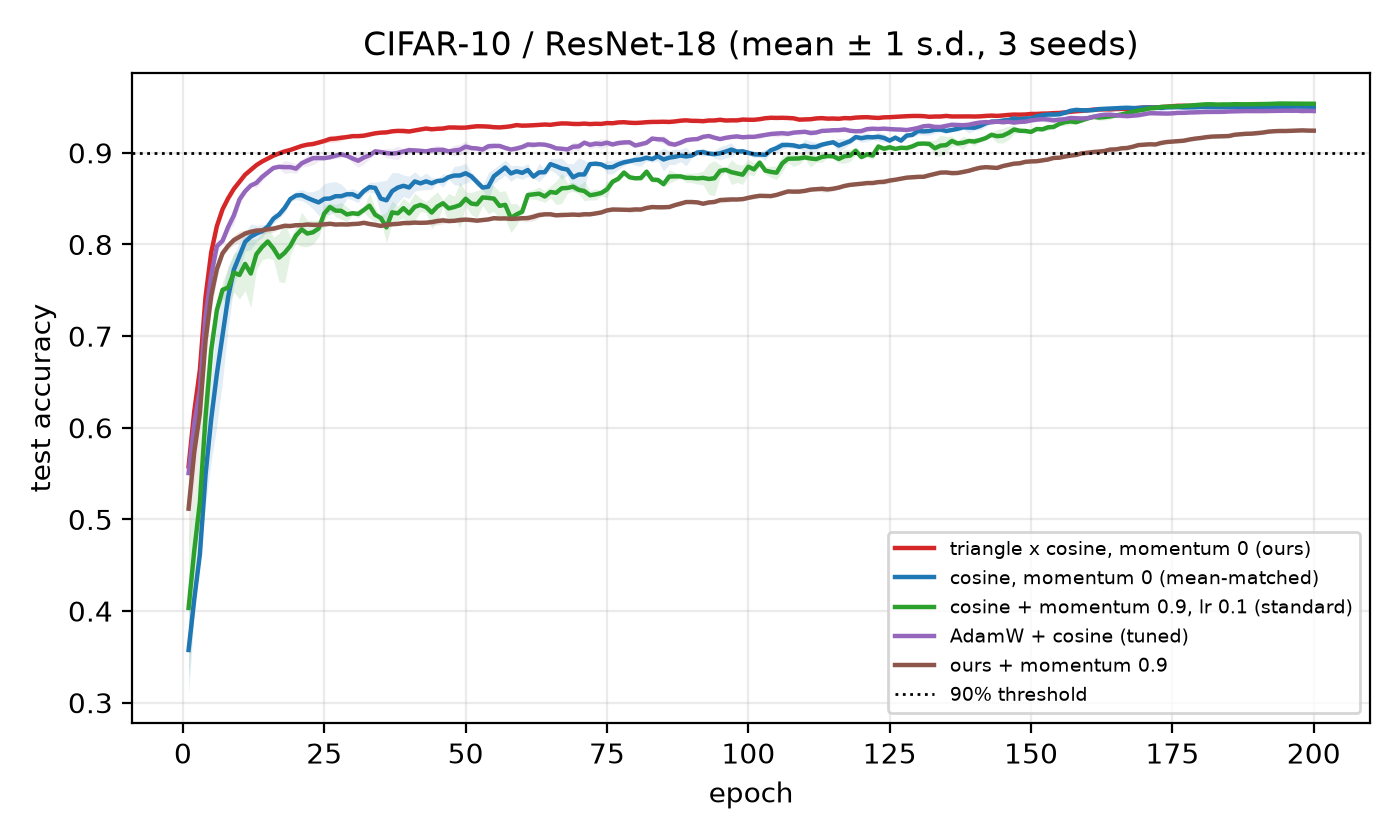
\includegraphics[width=0.92\linewidth]{figures/fig1_cifar10_accuracy.png}
\caption{Test accuracy on CIFAR-10/ResNet-18. Mean of 3 seeds (0, 1, 2), shaded $\pm 1$ s.d., 3-epoch moving average. The method (red) crosses 90\% at epoch \textasciitilde{}17. The standard momentum-0.9 recipe (green) needs \textasciitilde{}108 epochs to do the same. Applying the same schedule \textit{with} momentum (brown) is the worst arm in the figure; the mean-matched cosine control is blue and tuned AdamW is purple.}
\end{figure}

The method's mean learning rate is 0.200. A cosine anneal from peak 0.4 has mean 0.2000, so it differs from the method in exactly one way: no triangular cycle. This is the load-bearing control --- before it existed, the speed claim was measured against a baseline running at half the average step size.

\begin{center}
\small
\begin{tabular}{@{}lccccccc@{}}
\toprule
\textbf{arm} & \textbf{n} & \textbf{peak} & \textbf{final} & \textbf{t@90} & \textbf{t@93} & \textbf{t@94} & \textbf{t@95} \\
\midrule
\textbf{triangle x cosine} & 3 & \textbf{0.9526} & \textbf{0.9519} & \textbf{16.7} & \textbf{53} & \textbf{112} & 168 \\
cosine, peak 0.4 (mean-matched) & 3 & 0.9512 & 0.9504 & 68.7 & 132 & 149 & 166\dag \\
cosine, peak 0.2 & 3 & 0.9512 & 0.9507 & 44.3 & 114 & 134 & 171 \\
\bottomrule
\end{tabular}
\end{center}

\dag The mean-matched control's seed 2 peaks at 94.88\% and never reaches 95\%, so 166 is the mean of seeds 0-1 (165.5). The method reaches 95\% on 3/3 seeds.

Per-seed \texttt{t@90} (two-sided paired test, $n=3$): the method is 18/16/16 epochs, the mean-matched control 65/77/64. Paired difference \textbf{-52.0 epochs, $t=-11.53$, 3/3 seeds, 4.1x}. Final accuracy: +0.14 pp, $t=0.90$, not significant (and underpowered per \S{}4.2). The mean-matched control's larger seed spread (s.d. 7.2 epochs) is visible as the error bar at 90\% in Fig. 3.

The advantage is threshold-dependent and largest early: 4.1x at 90\%, 2.5x at 93\%, 1.3x at 94\%, and no significant gap at 95\% (\S{}5.2). Reporting only 90\% would be selective; the full curve is the result.

\begin{figure}[htbp]
\centering
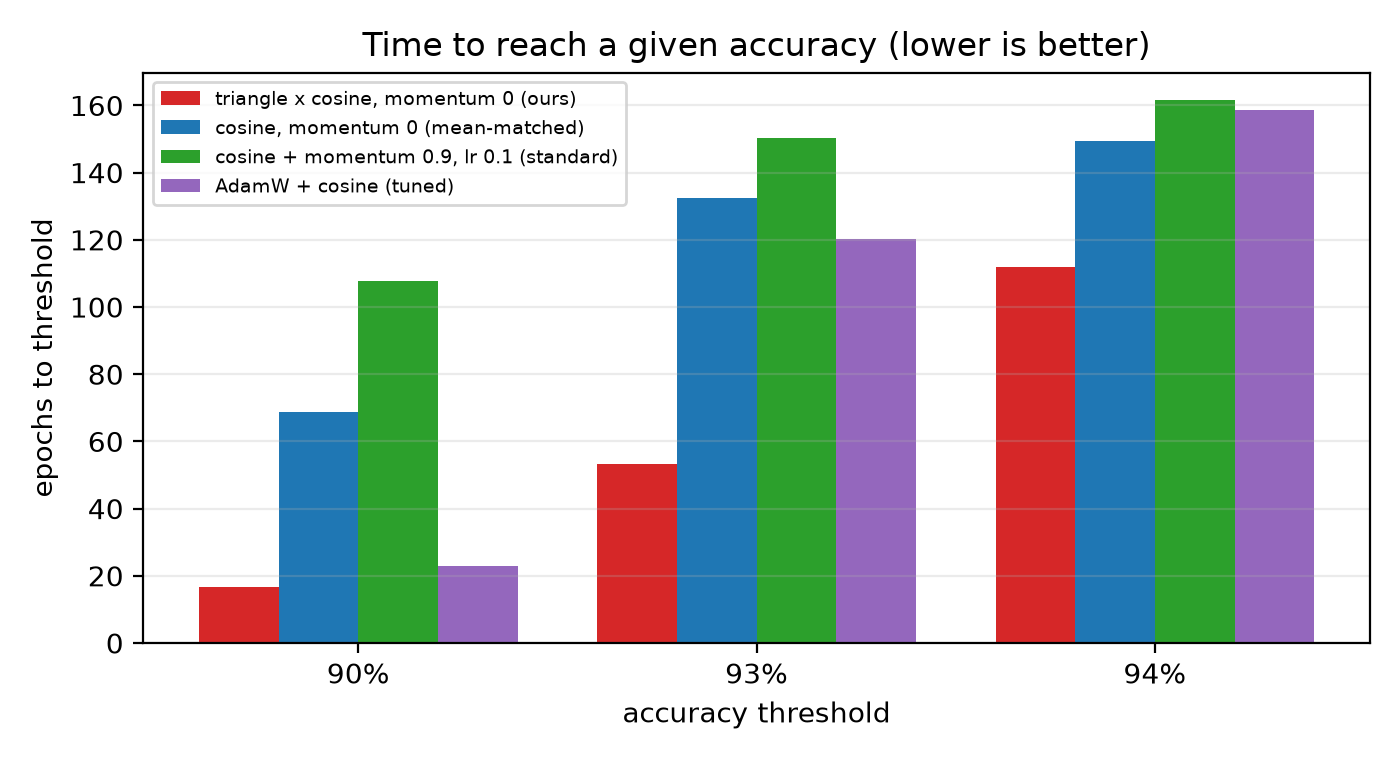
\includegraphics[width=0.92\linewidth]{figures/fig3_time_to_threshold.png}
\caption{Epochs required to reach 90/93/94\% test accuracy, with $\pm 1$ s.d. error bars across the three seeds. The method's bar is shortest at every threshold, and the gap narrows as the threshold approaches the accuracy ceiling. The same pattern appears on CIFAR-100 (\S{}5.6).}
\end{figure}

\subsection{The anytime profile: threshold and budget boundaries}
The effect is not a single number but a property of the accuracy-versus-epoch curve. Two boundaries bound it.

\textbf{Accuracy threshold.} The speedup is largest at the easiest threshold and disappears at the ceiling: 4.1x at 90\%, 2.5x at 93\%, 1.3x at 94\%, and no significant gap at 95\%. At 95\% the method takes 168 epochs on 3/3 seeds, while the mean-matched control reaches the threshold on only 2/3 seeds (the third peaks at 94.88\%); on the two common seeds the method is 2.5 epochs slower (n=2, t=0.71, not significant). On CIFAR-100 the same pattern holds (5.5x at 65\%, 5.3x at 70\%, a 3-seed tie at 75\%). This is the cleanest evidence that the schedule buys \textbf{convergence speed}, not a better optimum.

\textbf{Compute budget.} For each budget $B$ the anneal horizon is set to $B$ for every arm (1 seed; directional):

\begin{center}
\small
\begin{tabular}{@{}lcccc@{}}
\toprule
\textbf{budget} & \textbf{arm} & \textbf{t@90} & \textbf{final} & \textbf{peak} \\
\midrule
40 & triangle x cosine & \textbf{15} & \textbf{0.9324} & \textbf{0.9328} \\
40 & cosine, peak 0.2 & 21 & 0.9271 & 0.9271 \\
80 & triangle x cosine & \textbf{15} & \textbf{0.9445} & \textbf{0.9449} \\
80 & cosine, peak 0.2 & 30 & 0.9369 & 0.9395 \\
160 & triangle x cosine & \textbf{16} & \textbf{0.9496} & \textbf{0.9498} \\
160 & cosine, peak 0.2 & 45 & 0.9452 & 0.9455 \\
\bottomrule
\end{tabular}
\end{center}

The speed advantage is therefore not an artifact of holding the horizon at 200 epochs. Under a constrained budget the peak gap is also positive (+0.43 to +0.57 pp), shrinking to +0.14 pp at 200 epochs as the baseline catches up. The honest reading is the anytime one: when the budget is short, the schedule is both sooner and (directionally) higher; when the budget is long, the arms converge. The n=1 caveat means the peak ordering is a hypothesis, not a tested effect.

\subsection{Evaluation phase is not a confound}
Re-running the method with the cycle shifted by half an epoch, so validation lands on the LR peak rather than the trough: t@90 16 vs 17, t@93 53 vs 53, final 0.9522 vs 0.9519. All differences non-significant ($|t| \le 1.99$). The epoch-boundary alignment is therefore harmless, which also means the standard numbers can be reported as-is.

\subsection{Against the standard momentum recipe}
\begin{center}
\small
\begin{tabular}{@{}lccccc@{}}
\toprule
\textbf{arm} & \textbf{n} & \textbf{peak} & \textbf{final} & \textbf{t@90} & \textbf{t@93} \\
\midrule
\textbf{triangle x cosine, momentum 0} & 3 & 0.9526 & 0.9519 & \textbf{16.7} & \textbf{53} \\
cosine + momentum 0.9, lr 0.1 (standard) & 3 & \textbf{0.9543} & \textbf{0.9535} & 107.7 & 150 \\
cosine + momentum 0.9, lr 0.2 & 3 & 0.9500 & 0.9495 & 141.0 & 169 \\
triangle x cosine + momentum 0.9 & 3 & 0.9254 & 0.9236 & 159.0 & never \\
\bottomrule
\end{tabular}
\end{center}

Against the recipe a practitioner would actually run: \textbf{-91.0 epochs to 90\%, $t=-78.8$, 3/3 seeds (6.5x)}. Final accuracy is -0.17 pp ($t=-1.53$, not significant, and underpowered); \textbf{peak} accuracy is -0.16 pp ($t=-2.62$, 0/3 seeds) --- a consistent but very small deficit. The correct summary is ``reaches target accuracy far sooner, ends equal or a hair behind on final accuracy and a hair behind on peak''.

\subsection{Momentum-free is required, not incidental}
Adding momentum 0.9 to the method costs \textbf{2.82 pp final accuracy ($t=30.8$)} and \textbf{142 epochs to 90\% ($t=-213$)}, with all three seeds losing. The schedule at peak learning rate 0.8 does not survive momentum accumulation. This upgrades ``momentum-free'' from a description to a stated constraint, and it is consistent with the EoS account in \S{}6.2: without momentum the effective step is bounded by the instantaneous learning rate, and the triangular cycle keeps reinflating a step that is never accumulated.

\subsection{Second dataset: CIFAR-100}
\begin{figure}[htbp]
\centering
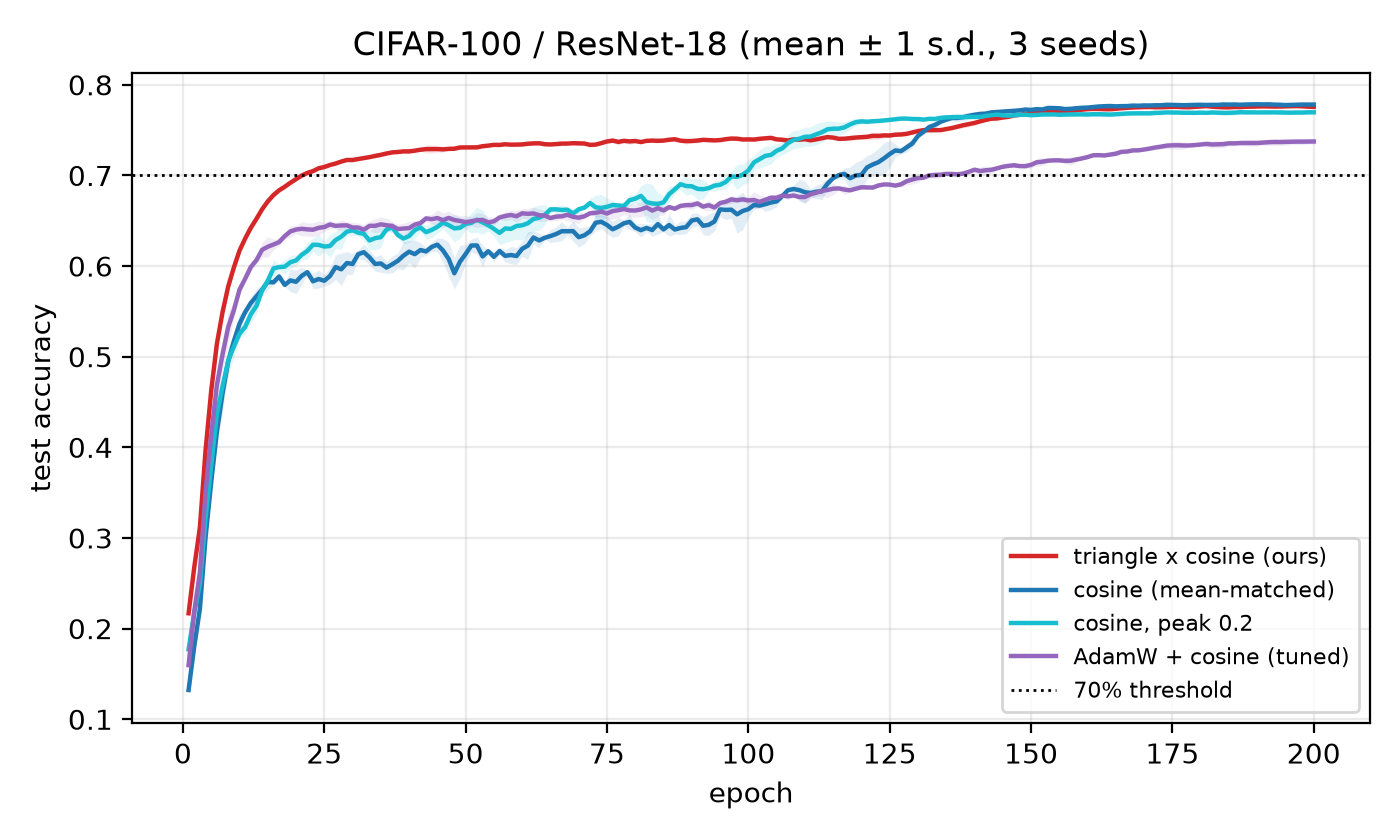
\includegraphics[width=0.92\linewidth]{figures/fig4_cifar100_accuracy.png}
\caption{CIFAR-100/ResNet-18, same protocol, mean of 3 seeds with $\pm 1$ s.d. bands. The method reaches 70\% at epoch \textasciitilde{}21 against \textasciitilde{}112 for the mean-matched cosine baseline, then the arms converge by epoch \textasciitilde{}130. The advantage lives in early-to-mid training on both datasets.}
\end{figure}

\begin{center}
\small
\begin{tabular}{@{}lccccc@{}}
\toprule
\textbf{arm} & \textbf{n} & \textbf{final} & \textbf{t@65} & \textbf{t@70} & \textbf{t@75} \\
\midrule
\textbf{triangle x cosine} & 3 & 0.7761 & \textbf{12.3} & \textbf{21.0} & 130.7 \\
cosine, peak 0.4 (mean-matched) & 3 & 0.7780 & 67.7 & 112.3 & 130.7 \\
cosine, peak 0.2 & 3 & 0.7695 & 39.7 & 89.7 & 111.7 \\
AdamW + cosine (lr 2e-3, wd 0.05) & 3 & 0.7373 & 33.7 & 129.0 & never \\
\bottomrule
\end{tabular}
\end{center}

Against the mean-matched control: t@65 \textbf{5.5x} ($t=-27.3$), t@70 \textbf{5.3x} ($t=-76.0$), final accuracy -0.20 pp ($t=-1.48$, not significant). Against AdamW: \textbf{+3.88 pp} ($t=38.2$, with the tuning caveat of \S{}5.7). The same threshold pattern appears: by 75\% the arms are identical (130.7 vs 130.7 epochs). Per-seed \texttt{t@65} is 12/13/12 for the method and 67/65/71 for the control, so the speed gap is not carried by one seed.

\subsection{AdamW}
Tuned over lr \{1e-3, 2e-3\} x wd \{0.01, 0.05\} on CIFAR-10, the best AdamW config reaches 0.9456 final against the method's 0.9519: \textbf{+0.63 pp, $t=6.37$, 3/3 seeds}. Against the previously reported untuned config the margin was +1.13 pp, so tuning halved it without removing it. Both lr and wd improve monotonically across the grid, so the optimum may lie beyond it; the claim is ``survives tuning'', not ``beats any tuned optimizer''. On CIFAR-100 the AdamW config was applied unchanged from CIFAR-10 (see \S{}7), so the +3.88 pp second-dataset margin is the least protected number in the paper. The cycle on AdamW is not beneficial: AdamW + cycle is -0.33 pp against AdamW + cosine ($t=-2.82$, not significant at $n=3$).

\subsection{Weight-decay conventions: a methodological result (E2)}
This experiment is reported in full because its lesson applies to any practitioner using a decaying learning rate, independently of the speed result. The question is simple: when the learning rate oscillates and anneals, what should the weight-decay coefficient multiply?

Three arms differ only in what the decay multiplies, with one literal \texttt{weight\_decay = 5e-4} for all of them:

\begin{center}
\small
\begin{tabular}{@{}>{\raggedright\arraybackslash}p{0.180\linewidth}>{\raggedright\arraybackslash}p{0.243\linewidth}>{\raggedright\arraybackslash}p{0.243\linewidth}>{\raggedright\arraybackslash}p{0.243\linewidth}@{}}
\toprule
\textbf{arm} & \textbf{decay factor} & \textbf{profile} & \textbf{mean shrink/step} \\
\midrule
B1 \texttt{wd x triangle x cosine} & oscillating \textbf{and} annealed & the method's convention & 1.0e-4 \\
B2 \texttt{wd x lr\_max x cosine} & smooth \textbf{and} annealed & decays with the anneal, no intra-epoch pulse & 2.0e-4 \\
F \texttt{wd} & constant & no LR scaling & 5.0e-4 \\
\bottomrule
\end{tabular}
\end{center}

\begin{figure}[htbp]
\centering
\includegraphics[width=0.92\linewidth]{figures/fig_e2_wd.png}
\caption{Left: test accuracy. B1 and B2 track each other; F is already below them at its peak and collapses in the tail. Right: mean weight norm. F keeps shrinking after the learning rate has annealed, ending near zero. Curves are mean and per-seed range over 3 seeds.}
\end{figure}

\begin{center}
\small
\begin{tabular}{@{}lcccccc@{}}
\toprule
\textbf{arm} & \textbf{peak acc} & \textbf{first 90\%} & \textbf{final acc} & \textbf{final loss} & \textbf{wnorm@50} & \textbf{wnorm@end} \\
\midrule
B1 effective & 0.9526 & 16.7 & 0.9519 & 0.194 & 39 & 24.3 \\
B2 base & \textbf{0.9534} & 18.3 & \textbf{0.9522} & 0.186 & 30.6 & 18.7 \\
F none & 0.9361 & 21.0 & \textbf{0.1030} & \textbf{2.3022} & 26.9 & \textbf{1.5} \\
\bottomrule
\end{tabular}
\end{center}

\textbf{Result 1 --- intra-epoch oscillation of the decay buys nothing.} B1 and B2 show no detectable difference: peak B2 - B1 = +0.077 pp ($t=0.91$) and final B2 - B1 = +0.033 pp ($t=0.24$), so B2 is nominally ahead on both means by a margin well inside seed noise. Once the decay anneals with the learning rate, whether it also pulses within the epoch does not matter.

\textbf{Result 2 --- in this run, an LR-independent decay coefficient collapsed to chance.} F ends at chance: final accuracy 0.1085 / 0.1000 / 0.1005 across the three seeds, and final loss 2.3022 for all three --- essentially $\ln 10 = 2.3026$ (the logged value is 2.3022), the entropy of a uniform prediction over ten classes. The collapse is abrupt and confined to the tail (seed 0):

\begin{center}
\small
\begin{tabular}{@{}lccccccc@{}}
\toprule
\textbf{epoch} & \textbf{150} & \textbf{170} & \textbf{185} & \textbf{190} & \textbf{195} & \textbf{198} & \textbf{200} \\
\midrule
val acc & 0.9245 & 0.9303 & \textbf{0.9362} & 0.9338 & 0.8645 & 0.5350 & \textbf{0.1085} \\
wnorm & 12.2 & 8.3 & 5.5 & 4.5 & 3.2 & 2.1 & \textbf{1.5} \\
\bottomrule
\end{tabular}
\end{center}

\textbf{Mechanism.} At epoch 199 the schedule's peak learning rate is \textasciitilde{}$1.3\times10^{-4}$ of its initial value, so gradient steps are negligible; F nevertheless keeps shrinking the weights by $5\times10^{-4}$ per step. Over the final epochs that is thousands of decay steps applied after learning has effectively stopped: the observed weight norm falls from 12.2 (epoch 150) to 1.5 (epoch 200), and the accuracy collapse follows it. B1 and B2 are protected because their multiplier decays to zero with the learning rate: at epoch 199 B1's per-step shrink is \textasciitilde{}$3\times10^{-10}$ and B2's \textasciitilde{}$1.6\times10^{-7}$.

What this run supports:

\begin{quote}
\textbf{In this setting, coupling decay to the learning rate --- in either form --- was sufficient to prevent the terminal collapse; a constant $5\times10^{-4}$ coefficient, also 2.5x/5x stronger on average, was not.}
\end{quote}

\textbf{Open confound (stated, not hidden).} F differs from B1/B2 in \textit{two} ways: constant profile \textbf{and} 2.5x/5x stronger average decay than B2/B1. Its peak accuracy is already 1.66 pp below B1 and 1.73 pp below B2 before any collapse, which is consistent with over-regularization throughout (a strength effect); the abrupt final collapse, coinciding with the LR reaching \textasciitilde{}1e-7, is consistent with a profile effect. The decisive strength-matched control --- F at \texttt{weight\_decay = 1e-4}, matching B1's mean shrink while keeping the constant profile --- was specified but not run. We therefore claim the safe version only: in this setting, both LR-coupled conventions survived the tail while the constant-coefficient arm did not, and smooth coupling is as effective as --- and simpler than --- oscillating coupling. We do \textbf{not} claim that the constant profile alone causes F's failure, nor that oscillating decay is better than smooth decay ($t=0.9$, not significant).

\textbf{Advice for training engineers.} (i) Do not assume that a literal \texttt{weight\_decay = 5e-4} under an annealed learning rate gives the same regularization as it does at constant LR: in our runs the constant-coefficient arm over-regularized at peak and collapsed in the tail. Prefer the framework's LR-scaled decay (torch's \texttt{SGD} default) or anneal the coefficient explicitly. (ii) You do not need to pulse weight decay at the LR cycle's frequency. (iii) Check the last few epochs' weight norm and loss; accuracy can look healthy until the collapse. Because strength and profile were confounded here, treat this as a strong caution rather than a proven mechanism.

\subsection{Ablations: what buys speed and what buys the final level}
\begin{itemize}
\item \textbf{Remove the anneal} (triangle only): still reaches 90\% at 16.7 epochs but caps at 0.9363 final --- the cycle buys the speed, the anneal supplies the final level.
\item \textbf{Constant learning rates} (6 values, 1 seed each): the best constant arm peaks at 0.9215 at lr 0.1, and every constant arm \textit{degrades} after its peak. No constant arm exceeds 92.2\% at its peak. This is the single most important control against ``it is just a learning rate'' and it is directional (n=1).
\item \textbf{Weight decay conventions}: see \S{}5.8.
\end{itemize}

\subsection{Loss and accuracy diverge}
On CIFAR-100 the method reaches the same accuracy at \textbf{significantly lower cross-entropy} (-0.0268, $t=-5.02$), while on CIFAR-10 both metrics are tied. The two metrics measure different things --- accuracy counts the argmax, cross-entropy scores the probability assigned to the true class --- so confidence can improve without the decision changing. We verified this is not an evaluation-phase artifact (\S{}5.3). Without a calibration metric we cannot separate better calibration from greater confidence on already-correct samples, so we report it as a secondary observation, not a claim.

\section{Discussion}
\subsection{Anytime efficiency, not accuracy superiority}
The result is best understood as an \textbf{anytime} property. Given a fixed compute budget, the schedule delivers a usable model sooner; given a budget large enough for both to converge, it delivers the same model. The effect is therefore about the \textit{shape of the accuracy-versus-epoch curve} in early-to-mid training, not about the endpoint. This is the only framing in which the result is both true and useful: practitioners who care about time-to-accuracy --- hyperparameter search, early stopping, limited budgets --- get several times more throughput per unit of training, while practitioners who care only about the final number should use the standard momentum recipe, which is marginally more accurate on peak.

We explicitly do not claim that the schedule is superior over long training horizons. At 200 epochs the arms show no detectable difference on final accuracy, and the momentum recipe is 0.16 pp ahead on peak. The defensible claim is narrower: \textbf{inside a fixed budget, and before the ceiling is reached, the cycle is a more efficient use of training time}.

\subsection{A candidate mechanism at the edge of stability}
Two mechanisms are consistent with our ablations and we do not claim to separate them fully: (i) the cycle repeatedly depresses the learning rate to the floor, letting the model settle at many points during training rather than only at the end; (ii) the high peak explores faster while the short depression bounds the damage. The momentum result (\S{}5.5) supports (ii): momentum would carry the high-learning-rate step into the low-learning-rate phase.

EoS supplies a sharper version of (ii). If the sharpness of the loss sits near the stability threshold $2/\eta$, then a schedule that varies $\eta$ over three orders of magnitude within each epoch is not merely ``sometimes large, sometimes small'': it is repeatedly pushing the optimizer across the EoS boundary. The high-$\eta$ phase can progressively sharpen and explore, and the low-$\eta$ phase damps the resulting excursions --- the pattern EoS work associates with non-monotone short-timescale loss but long-timescale descent \cite{ref6,ref7,ref8}. In this reading the one-epoch cycle acts as a high-frequency probe of the stability boundary, which is why it accelerates early learning but cannot beat the ceiling: it changes the path, not the minimum.

This account makes a falsifiable prediction, which we have not tested: the effect should weaken as the peak learning rate is lowered toward the stable regime, and sharpness ($\lambda_{\max}$) should trace a sawtooth locked to the cycle. A sharpness-trajectory experiment --- $\lambda_{\max}$ versus $2/\eta(t)$ --- is the natural next step \cite{ref6}, and it would turn the EoS framing from an analogy into a measurement. Two caveats keep this section honest: EoS theory is stated for fixed-step, full-batch GD, while we run mini-batch SGD with a time-varying step; and we did not measure Hessian spectra in this work.

\subsection{The boundary map}
The contribution is as much about where the effect stops as where it starts:

\begin{center}
\small
\begin{tabular}{@{}>{\raggedright\arraybackslash}p{0.180\linewidth}>{\raggedright\arraybackslash}p{0.243\linewidth}>{\raggedright\arraybackslash}p{0.243\linewidth}>{\raggedright\arraybackslash}p{0.243\linewidth}@{}}
\toprule
\textbf{dimension} & \textbf{range tested} & \textbf{effect present} & \textbf{effect absent / untested} \\
\midrule
accuracy threshold & CIFAR-10 90-95\%; CIFAR-100 65-75\% & 90-93\% (4.1x, 2.5x); 65-70\% (5.5x, 5.3x) & at the ceiling: 95\% has no significant gap (control reaches it on 2/3 seeds); 75\% is a 3-seed tie \\
training budget & 40, 80, 160, 200 epochs & speed at every budget; peak gap +0.43 to +0.57 pp at 40-160 & peak gap shrinks to +0.14 pp at 200 \\
momentum & 0 vs 0.9 & momentum-free only & with momentum 0.9: 2.8 pp worse, 142 epochs slower \\
optimizer & SGD vs AdamW & momentum-free SGD & AdamW: no detectable benefit at the tested config (-0.33 pp, n.s.) \\
dataset & CIFAR-10, CIFAR-100 & replicates on both & untested on other data \\
architecture / resolution & ResNet-18, 32x32 & this setting only & untested at ImageNet scale, higher resolution, transformers \\
peak learning rate & 0.8 only & 0.8 & 0.4 and 1.2 not run \\
cycle period & 1 epoch only & 1 epoch & no period sweep; a growing-period pilot was ambiguous and is not a paper claim \\
\bottomrule
\end{tabular}
\end{center}

The map is the paper's honest core. A practitioner can read it as a decision rule: use the cycle when the budget is short, the target is below the ceiling, the optimizer is momentum-free SGD, and the model is a small-data vision CNN; otherwise use a standard annealed recipe.

\subsection{Practical guidance}
\begin{enumerate}
\item \textbf{Short budgets and hyperparameter search.} The schedule is worth trying when you will stop well before convergence or when you need a usable checkpoint early. It is not worth trying if you will train to the ceiling and only care about the final number.
\item \textbf{Do not add momentum.} The effect is momentum-free by construction; momentum both destroys it and makes the high peak unsafe.
\item \textbf{Do not leave weight decay LR-independent.} This is the one piece of advice in the paper that applies to schedules other than ours. In \S{}5.8 a constant coefficient collapsed in the tail while LR-coupled decay did not, although profile and strength were confounded; treat it as a strong caution and check your framework's convention.
\item \textbf{Report time-to-threshold as well as final accuracy.} A schedule can be anytime-better while asymptotically equal, and a final-number-only report would miss the entire effect.
\end{enumerate}

\subsection{What would change our mind}
The claims above are falsifiable and we name the experiments that could break them: a peak-LR sweep at 0.4 and 1.2 (if the result is a knife-edge at 0.8, the practical claim weakens); a per-budget retune of the cosine baseline (if the constrained-budget peak advantage disappears, that sub-claim goes); a CIFAR-100 AdamW grid (if AdamW reaches \textasciitilde{}0.76, the +3.88 pp margin shrinks toward the CIFAR-10 figure); and seeds 3 $\to$ 5 on the headline arms (which would tighten the underpowered final-accuracy ties). None of these can invalidate H1-H4; the first two are the most likely reviewer requests.

\section{Limitations and threats to validity}
We list these as strengths of the evidence, not as an apology: each is a boundary the paper knowingly does not cross.

\begin{itemize}
\item \textbf{Scale.} One architecture (ResNet-18) and two datasets, both 32x32 with a \textasciitilde{}50k-image training set. The regime is untested on ImageNet-scale data, higher input resolutions, or transformers (which require warmup \cite{ref5} and would not tolerate peak 0.8 from step 0).
\item \textbf{Peak learning rate was inherited, not tuned.} 0.8 came from earlier work; the sensitivity sweep at 0.4 and 1.2 has not been run. This is why the title makes no robustness claim about the configuration space.
\item \textbf{AdamW was not tuned on CIFAR-100.} The winning CIFAR-10 config (lr 2e-3, wd 0.05) was applied unchanged; two CIFAR-100 AdamW points exist (0.7283, n=1; 0.7373, n=3), both well below the method's 0.7761, so the direction is consistent, but a per-dataset optimum could shrink the +3.88 pp margin toward the CIFAR-10 figure. The AdamW grid may also not contain the optimum (both lr and wd improved monotonically across it).
\item \textbf{Tuning on the test split.} All arms are tuned on the CIFAR-10 test split rather than a validation split. The practice is symmetric across arms, so no arm is advantaged relative to the others, but it is not standard and a validation split should be carved out before submission.
\item \textbf{Seed count.} Headline arms use $n=3$, which underpowers differences below \textasciitilde{}0.6-0.8 pp. Consequently the final-accuracy ties are ``no detectable difference'', not proven equality. Seeds 3 $\to$ 5 would tighten them.
\item \textbf{Single-seed arms.} The budget-matched runs and the constant-LR sweep are $n=1$; their results are directional only.
\item \textbf{Weight-decay confound.} In E2 the constant-decay arm differs in both profile and strength; the strength-matched control was specified but not run (\S{}5.8).
\item \textbf{No period sweep and no step-decay baseline.} A growing-period pilot was ambiguous and is not reported as a claim. A step-decay baseline would be a standard comparison a reviewer may request.
\item \textbf{No sharpness measurement.} The EoS account in \S{}6.2 is an interpretive hypothesis, not a measured mechanism.
\end{itemize}

\section{Reproducibility}
Code, configs and per-run JSONs are in the repository. Headline, AdamW, CIFAR-100 and budget tables are regenerated by \texttt{python scripts/weekend\_report.py}; the E2 table by \texttt{python scripts/summarize\_e2.py}; figures by \texttt{python scripts/make\_figures.py} (Figs. 1-4) and \texttt{python scripts/plot\_e2.py} (Fig. 5). Runs are resumable (\texttt{--skip-existing}) and take \textasciitilde{}20 s/epoch on a single RTX A4000. The method is stock PyTorch (\texttt{SGD} + \texttt{LambdaLR}); no custom optimizer is in the method path. The schedule is two lines, reproduced in \S{}3.1. Seeds are fixed at 0, 1, 2 for all paired comparisons; per-seed values are retained in the JSONs so every mean, s.d. and paired test in this paper can be recomputed from the raw run histories.

\section{Conclusion}
We characterised a schedule that is deliberately unoriginal --- Smith's triangular cycle at a one-epoch period multiplied by a cosine anneal --- in a regime the literature has not isolated. In a fixed 200-epoch budget it reaches target accuracies several times sooner than mean-matched cosine and standard momentum recipes, at final accuracy with no detectable difference; it does so only for momentum-free SGD, only below each dataset's ceiling, and only on the small-data vision setting we tested. It does not improve the endpoint, and we do not claim that it does. Along the way, two negative results are worth keeping: adding momentum destroys the effect, and in our runs a constant weight-decay coefficient under an annealed learning rate collapsed to chance while LR-coupled decay did not (with the strength confound noted). The honest headline is therefore \textbf{faster, not better}, with the boundaries stated.

\begin{thebibliography}{14}
\bibitem{ref1} L. N. Smith. Cyclical learning rates for training neural networks. WACV 2017. arXiv:1506.01186. \url{https://arxiv.org/abs/1506.01186}

\bibitem{ref2} I. Loshchilov and F. Hutter. SGDR: Stochastic gradient descent with warm restarts. ICLR 2017. arXiv:1608.03983. \url{https://arxiv.org/abs/1608.03983}

\bibitem{ref3} L. N. Smith and N. Topin. Super-convergence: Very fast training of neural networks using large learning rates. arXiv:1708.07120. \url{https://arxiv.org/abs/1708.07120}

\bibitem{ref4} L. N. Smith. A disciplined approach to neural network hyper-parameters: Part 1. arXiv:1803.09820. \url{https://arxiv.org/abs/1803.09820}

\bibitem{ref5} P. Goyal et al. Accurate, large minibatch SGD: training ImageNet in 1 hour. arXiv:1706.02677. \url{https://arxiv.org/abs/1706.02677}

\bibitem{ref6} J. M. Cohen, S. Kaur, Y. Li, J. Z. Kolter, A. Talwalkar. Gradient descent on neural networks typically occurs at the edge of stability. ICLR 2021. arXiv:2103.00065. \url{https://arxiv.org/abs/2103.00065}

\bibitem{ref7} S. Jastrz\k{e}bski et al. The break-even point on optimization trajectories of deep neural networks. arXiv:2002.09572. \url{https://arxiv.org/abs/2002.09572}

\bibitem{ref8} Good regularity creates large learning rate implicit biases: edge of stability, balancing, and catapult. JMLR 26 (2025). \url{https://dl.acm.org/doi/10.5555/3814246.3814519}

\bibitem{ref9} A. H\"agele et al. Scaling laws and compute-optimal training beyond fixed training durations. NeurIPS 2024. arXiv:2405.18392. \url{https://arxiv.org/abs/2405.18392}

\bibitem{ref10} Understanding warmup-stable-decay learning rates: a river valley loss landscape perspective. ICLR 2025. arXiv:2410.05192. \url{https://arxiv.org/abs/2410.05192}

\bibitem{ref11} Y. Shen et al. Power scheduler: a batch-size and token-count agnostic learning rate scheduler. arXiv:2408.13359. \url{https://arxiv.org/abs/2408.13359}

\bibitem{ref12} X. Liu and Y. Ma. The epochal sawtooth phenomenon: unveiling training loss oscillations in Adam and other optimizers. arXiv:2410.10056. \url{https://arxiv.org/abs/2410.10056}

\bibitem{ref13} A. Krizhevsky. Learning multiple layers of features from tiny images. Technical report, University of Toronto, 2009.

\bibitem{ref14} K. He, X. Zhang, S. Ren, J. Sun. Deep residual learning for image recognition. CVPR 2016. arXiv:1512.03385. \url{https://arxiv.org/abs/1512.03385}

\end{thebibliography}

\appendix
\section{Statistical details}
Paired tests use the per-seed difference between arms on the same seed (shared initialization and data order). For $n=3$ pairs, the two-sided critical value is $|t| \ge 4.303$ at $\alpha = 0.05$. The minimum detectable effect at 80\% power is approximately $2.84 \times \mathrm{sd}_\text{paired}$; at a paired s.d. of 0.2 pp on accuracy this is \textasciitilde{}0.6 pp, and for the headline mean-matched tie (paired s.d. 0.28 pp) it is \textasciitilde{}0.8 pp. Sub-resolution accuracy differences are reported as ``no detectable difference''. Time-to-threshold differences are much larger than this floor (e.g. 52 epochs with a paired s.d. of \textasciitilde{}8), so their tests are well powered.

\begin{center}
\footnotesize
\setlength{\tabcolsep}{3pt}
\begin{tabular}{@{}lccccc@{}}
\toprule
\textbf{comparison} & \textbf{metric} & \textbf{effect} & \textbf{t} & \textbf{seeds} & \textbf{verdict} \\
\midrule
method vs mean-matched cosine & t@90 & -52.0 ep (4.1x) & -11.53 & 3/3 & significant \\
method vs mean-matched cosine & final acc & +0.14 pp & +0.90 & 2/3 & n.s. (underpowered) \\
method vs standard momentum recipe & t@90 & -91.0 ep (6.5x) & -78.81 & 3/3 & significant \\
method vs standard momentum recipe & final acc & -0.17 pp & -1.53 & 1/3 & n.s. (underpowered) \\
method vs standard momentum recipe & peak acc & -0.16 pp & -2.62 & 0/3 & consistent small deficit \\
method vs method + momentum & final acc & +2.82 pp & +30.78 & 3/3 & significant \\
method vs tuned AdamW & final acc & +0.63 pp & +6.37 & 3/3 & significant \\
B2 vs B1 (smooth vs oscillating decay) & peak acc & +0.077 pp & +0.91 & 2/3 & n.s. \\
B2 vs B1 (smooth vs oscillating decay) & final acc & +0.033 pp & +0.24 & 2/3 & n.s. \\
\bottomrule
\end{tabular}
\end{center}

\end{document}
